\begin{figure}
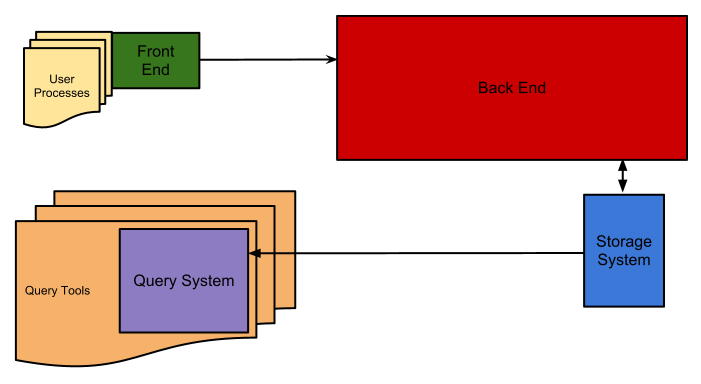
\includegraphics[width=\textwidth]{BroadProvDesign.png}
\label{fig:broaddes}
\caption{Broad design of the provenance system.}
\end{figure}
The system will consist of four main parts.
\begin{enumerate}
\item A front end which captures provenance data from the users activities.
\item A back end which processes raw provenance data into related provenance objects.
\item A self contained storage system which persists provenance objects.
\item A query API which will return provenance objects to user tools.
\end{enumerate}
The system will be designed such that it would be possible to run several instances of front end systems simultaneously.

In our initial implementation we are planning to use a libC based system call interception technique in our front end to capture user provenance data transparently and with low overhead. We are planning to use a local key/value store for our initial storage system.
